\documentclass{article}

\usepackage[utf8]{inputenc}

\usepackage{nicefrac}
\usepackage{amssymb, amsmath, amsfonts}
\usepackage{amsthm}
\usepackage{tikz}
\usetikzlibrary{matrix,shapes,arrows, calc, intersections}
\usepackage{pgfplots}
\usepgfplotslibrary{groupplots}
\usepackage[a4paper, margin=1in]{geometry}

\newtheorem{proposition}{Proposition}
\newtheorem{theorem}{Theorem}
\newtheorem{definition}{Definition}
\newtheorem{lemma}{Lemma}
\newtheorem{conjecture}{Conjecture}
\newtheorem{corollary}{Corollary}
\newtheorem{remark}{Remark}
\newtheorem{assumption}{Assumption}

\newlength\figureheight
\newlength\figurewidth
\setlength\figureheight{12cm}
\setlength\figurewidth{14cm}

\newcommand{\tikzdir}[1]{tikz/#1.tikz}
\newcommand{\inputtikz}[1]{\input{\tikzdir{#1}}}

\DeclareMathOperator*{\argmin}{arg\; min}     % argmin
\DeclareMathOperator*{\argmax}{arg\; max}     % argmax
\DeclareMathOperator*{\tr}{tr}     % trace
\DeclareMathOperator{\Cov}{Cov}
\DeclareMathOperator{\logdet}{log\;det}

\title{EE8087 Living with Mathematics\\Quiz 1}
\date{}
\begin{document} \maketitle
\begin{enumerate}
\item  An engineer determines that the angle of elevation from her position to the top of a tower is $60^\circ$ . She measures the angle of elevation again from a point $60$m further away from position and finds it to be $30^\circ$ . Both positions are due east of the tower. Find the height of the tower.

   \begin{figure}[ht]
    \centering
    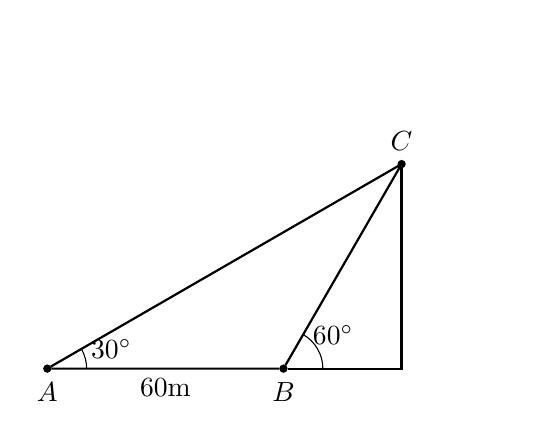
\begin{tikzpicture}[scale=0.5]
      \tikzset{mark coordinate/.style={inner sep=0pt,
          outer sep=0pt,
          minimum size=3pt,
          fill=#1,
          circle}
      }
      \node [mark coordinate=black,label=270:$A$] (A) at (0,0) {}; 
      \node [mark coordinate=black,label=270:$B$] (B) at (6,0) {}; 
      \coordinate (A1) at ($(A)+(30:14)$);
      \coordinate (B1) at ($(B)+(60:10)$);
      \path [name path=AC] (A)--(A1);
      \path [name path=BC] (B)--(B1);
      \path [name intersections={of=AC and BC, by=C}];
      \node [mark coordinate=black, label=90:$C$] at (C) {};
      \draw [thick] (A)--(C)--(B)--node [below]{$60$m} (A);
      \draw [thick] (C)|-(B);

      \draw (1,0) arc (0:30:1) node [right] {$30^\circ$};
      \draw (7,0) arc (0:60:1) node [right] {$60^\circ$};

    \end{tikzpicture}
  \end{figure}
\emph{Soln:} Suppose the vertical distance from $B$ to $C$ is $h$ and the horizontal distance is $d$. Hence, we have
\begin{align*}
  d = h \tan 60^\circ,\, (d+60)=h\tan 30^\circ.
\end{align*}
Therefore, $d = 30$m and $h = 30\sqrt{3}$m.

\newpage

\item Consider a parabola with focus $F$ and vertex $V$ and $FV = 1$. Suppose $P$ and $Q$ are two points on the parabola, such that $P$, $F$ and $Q$ are colinear. Furthermore, $\angle VFP = 120^\circ$. Find the length of $PQ$.

\begin{figure}[h]
  \centering
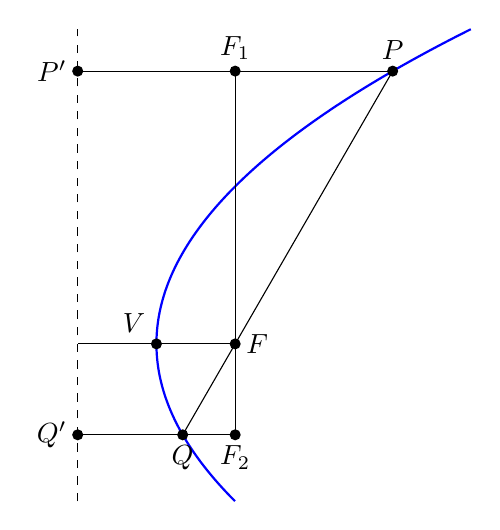
\begin{tikzpicture}
  \draw[domain=0:2, samples=200,smooth,variable=\t,blue,thick] plot ({\t*\t},{2*\t)});
  \draw[domain=0:1, samples=200,smooth,variable=\t,blue,thick] plot ({\t*\t},{-2*\t)});
  \coordinate (O) at (-1,0);
  \draw [dashed] (-1,-2)--(-1,4);
  \node [inner sep=0, outer sep=0, label=0:$F$] (F) at (1,0) {}; 
  \fill [black] (F) circle (2pt); 
  \node [inner sep=0, outer sep=0, label=135:$V$] (V) at (0,0) {}; 
  \fill [black] (V) circle (2pt); 
 
  \node [inner sep=0, outer sep=0, label=90:$P$] (P) at (3,{2*sqrt(3)}) {}; 
  \fill [black] (P) circle (2pt); 
  \node [inner sep=0, outer sep=0, label=270:$Q$] (Q) at ({1/3},{-2/sqrt(3)}) {}; 
  \fill [black] (Q) circle (2pt); 
  \draw (P)--(Q);
  \draw (F)--(O);

  \draw (P)--(P-|O);
  \node [inner sep=0, outer sep=0, label=180:$P'$] (PP) at (P-|O) {}; 
  \fill [black] (PP) circle (2pt); 

  \draw (Q)--(Q-|O);
  \node [inner sep=0, outer sep=0, label=180:$Q'$] (QQ) at (Q-|O) {}; 
  \fill [black] (QQ) circle (2pt); 


  \draw (F)|-(P);
  \node [inner sep=0, outer sep=0, label=90:$F_1$] (F1) at (F|-P) {}; 
  \fill [black] (F1) circle (2pt); 

  \draw (F)|-(Q);
  \node [inner sep=0, outer sep=0, label=270:$F_2$] (F2) at (F|-Q) {}; 
  \fill [black] (F2) circle (2pt); 
\end{tikzpicture}
\end{figure}
\emph{Soln:} Since $FV = 1$, we know that the distance from $F$ to the directrix is $2$. 

Find $P'$ and $Q'$ on the directrix such that $PP'$ and $QQ'$ are perpendicular to the directrix.

Suppose $FP = r_1$ and $FQ = r_2$. From the definition of parabola, we know that 

\begin{align*}
 PP' = FP = r_1,\,QQ' = FQ = r_2. 
\end{align*}
On the other hand,
\begin{align*}
  PP' &= P'F_1 + F_1 P = 2 + r_1\sin 30^\circ = 2+0.5r_1,\\
  QQ' &= Q'F_2 - F_2 Q = 2 - r_2\sin 30^\circ = 2-0.5r_2.
\end{align*}

Therefore, we can solve $r_1 = 4$ and $r_2 = 4/3$. Hence, $PQ = r_1+r_2 = 16/3$.

\newpage

\item Find the maximum value of $\sin x + \cos x$.

\emph{Soln:} \begin{align*}
               \sin x + \cos x = \sqrt{2} \left(\sin x\cos 45^\circ + \cos x \sin 45^\circ \right) = \sqrt{2} \sin (x + 45^\circ).
             \end{align*}
             Therefore, the maximum value is $\sqrt{2}$.

\newpage
\item Suppose we have two paper strips $OP$ and $PQ$ that are connected at point $P$. Furthermore $OP = PQ = 1$. Let $R$ be the middle point of $PQ$.
  
Suppose that $O$ is fixed at the origin and $Q$ is moving along the $x$-axis. If $\angle POQ = \theta$, derive the coordinate of $R$ and write down the quadratic equation describing the trajectory of $R$.
\begin{figure}[ht]
  \centering
  \begin{tikzpicture}[scale=2]
 \draw[->] (-2,0) -- (2,0) node[right] {$x$};
  \draw[->] (0,-1) -- (0,1) node[above] {$y$};

  \node [inner sep=0, outer sep=0, label=90:$P$] (P) at (30:1) {}; 
  \fill [black] (P) circle (1pt); 

  \node [inner sep=0, outer sep=0, label=90:$Q$] (Q) at ({sqrt(3)},0) {}; 
  \fill [black] (Q) circle (1pt); 

  \node [inner sep=0, outer sep=0, label=225:$O$] (O) at (0,0) {}; 
  \fill [black] (O) circle (1pt); 

  \node [inner sep=0, outer sep=0, label=90:$R$] (R) at ({sqrt(3)*0.75}, {0.25}) {}; 
  \fill [black] (R) circle (1pt); 
  
\draw [thick] (O)--(P)--(Q);
\draw (0.2,0) arc (0:30:0.2) node [right] {$\theta$};

  \end{tikzpicture}
\end{figure}

\emph{Soln:} The coordinate of $P$ is $(\cos \theta, \sin \theta)$ and the coordinate of $Q$ is $(2\cos\theta, 0)$. As a result, 
\begin{align*}
  R = (P+Q)/2 = (1.5\cos\theta, 0.5\sin\theta).
\end{align*}
Hence, $R$ is on the following ellipse:
\begin{align*}
  \frac{x^2}{1.5^2}+\frac{y^2}{0.5^2} = 1.
\end{align*}




\end{enumerate}

\end{document}
%%% Local Variables:
%%% TeX-command-default: "Latexmk"
%%% End:
